%%%%%%%%%%%%%%%%%%%%%%%%%%%%%%%%%%%%%%%%%
% Short Sectioned Assignment
% LaTeX Template
% Version 1.0 (5/5/12)
%
% This template has been downloaded from:
% http://www.LaTeXTemplates.com
%
% Original author:
% Frits Wenneker (http://www.howtotex.com)
%
% License:
% CC BY-NC-SA 3.0 (http://creativecommons.org/licenses/by-nc-sa/3.0/)
%
%%%%%%%%%%%%%%%%%%%%%%%%%%%%%%%%%%%%%%%%%

%----------------------------------------------------------------------------------------
%	PACKAGES AND OTHER DOCUMENT CONFIGURATIONS
%----------------------------------------------------------------------------------------

\documentclass[paper=letter, fontsize=11pt]{scrartcl} % A4 paper and 11pt font size

\usepackage[T1]{fontenc} % Use 8-bit encoding that has 256 glyphs
%\usepackage{fourier} % Use the Adobe Utopia font for the document - comment this line to return to the LaTeX default
\usepackage[english]{babel} % English language/hyphenation
\usepackage{amsmath,amsfonts,amsthm} % Math packages

\usepackage{enumitem}

\usepackage{sectsty} % Allows customizing section commands

%these two packages are needed for xfig 
\usepackage[dvips,final]{graphicx}
\usepackage{color} %include even if images aren’t in color

\usepackage{float}
\floatstyle{boxed} 
\restylefloat{figure}


\allsectionsfont{\centering \normalfont\scshape} % Make all sections centered, the default font and small caps

\usepackage{fancyhdr} % Custom headers and footers
\pagestyle{fancyplain} % Makes all pages in the document conform to the custom headers and footers
\fancyhead{} % No page header - if you want one, create it in the same way as the footers below
\fancyfoot[L]{} % Empty left footer
\fancyfoot[C]{\thepage} % Empty center footer
\fancyfoot[R]{} % Page numbering for right footer
\renewcommand{\headrulewidth}{0pt} % Remove header underlines
\renewcommand{\footrulewidth}{0pt} % Remove footer underlines
\setlength{\headheight}{13.6pt} % Customize the height of the header

%\numberwithin{equation}{section} % Number equations within sections (i.e. 1.1, 1.2, 2.1, 2.2 instead of 1, 2, 3, 4)
%\numberwithin{figure}{section} % Number figures within sections (i.e. 1.1, 1.2, 2.1, 2.2 instead of 1, 2, 3, 4)
%\numberwithin{table}{section} % Number tables within sections (i.e. 1.1, 1.2, 2.1, 2.2 instead of 1, 2, 3, 4)

\setlength\parindent{0pt} % Removes all indentation from paragraphs - comment this line for an assignment with lots of text

%----------------------------------------------------------------------------------------
%	TITLE SECTION
%----------------------------------------------------------------------------------------

\newcommand{\horrule}[1]{\rule{\linewidth}{#1}} % Create horizontal rule command with 1 argument of height

\title{	
\normalfont \normalsize 
\textsc{University of Lethbridge} \\ [25pt] % Your university, school and/or department name(s)
\horrule{0.5pt} \\[0.4cm] % Thin top horizontal rule
\huge Computational Optimization Term Project Report\\ % The assignment title
\horrule{2pt} \\[0.5cm] % Thick bottom horizontal rule
}

\author{Ahamad Imtiaz Khan\\ID:001188188} % Your name

\date{\normalsize\today} % Today's date or a custom date

\begin{document}

\maketitle % Print the title

%----------------------------------------------------------------------------------------
%	PROBLEM 1
%----------------------------------------------------------------------------------------
\begin{center}
\LARGE Problem 1
\end{center}

\Large \textbf{1. Problem Statement:}
\normalsize Sarah is an Operation Management Student of Takshashila University (TU). In her 
last semester she will need to take some courses.Some courses are compulsory as some courses have choices.
For choosing the courses Sarah need to fulfil some conditions.They are stated as bellow:
    
\begin{enumerate} [align=left,style=nextline,leftmargin=1.5cm,labelsep=\parindent,font=\normalfont]
\item[i.] She has to take 5 courses in total.
\item[ii.] She has to take Business Strategy (MGT 490) and International Finance (FIN 358).
\item[iii.] She has interest in service-learning course and found Intergenerational Computing (CIS 102T) and Web Design for Non-profit Organizations (CIS 102W) interesting. She will take one of the two courses 
between these.
\item[iv.] Between four potential finance elective courses (Data Analysis in Finance (FIN 325),
 Risk Management(FIN 352), Options, Futures, and Swaps (FIN 356) and 
Fixed Instruments and Markets (FIN 359)) she will take two courses.
\end{enumerate}

Sarah rated each section of the available courses based on content of the course, reputation of the instructor and timing of the course. Now it's my job to find an appropriate schedule for Sarah which will meet all the above mentioned conditions and also will give highest total rating. I will solve the problem using two strategies. First one is Greedy Heuristic and the second one is LP model. Using Greedy Heuristic I will find a solution which may not be optimal but good enough, using LP model I will find optimal solution and finally I will find maximum rating of three days a week schedule by extending the LP .\\
\newline
\Large \textbf{2. Input Data:}
\normalsize The input data for the problem are rearranged as follows: 

\begin{table}[h]
\begin{center}
    \resizebox{\textwidth}{!}{\begin{tabular}{| l | l | l | l | l | l | l | l | l |}
  
    \hline
    Meeting Time(s) & MGT 490 & FIN 358 & CIS 102T & CIS 102W & FIN 325 & FIN 352 & FIN 356 & FIN 359 \\ \hline
    M 6-8:45 p.m. & 4.3 & 0 & 0 & 0 & 0 & 3.6 & 0 & 3 \\ \hline
    T 6-8:45 p.m. & 3.8 & 0 & 0 & 3.7 & 0 & 0 & 3.2 & 0 \\ \hline
    W 6-8:45 p.m. & 3.5 & 3.5 & 0 & 0 & 0 & 0 & 0 & 3.5 \\ \hline
    F 6-8:45 p.m. & 3.5 & 0 & 0 & 0 & 0 & 0 & 0 & 0 \\ \hline
    \shortstack[l]{M 1:25-2:20 p.m. \\ W 1:25-3:15 p.m.} & 4.6 & 0 & 0 & 0 & 3.7 & 0 & 0 & 0 \\ \hline
    \shortstack[l]{T 1:25-3:15 p.m. \\ Th 1:25-2:20 p.m.} & 2.7 & 3.3 & 0 & 0 & 0 & 0 & 3.4 & 0 \\ \hline
    W 2:30-5:15 p.m. & 0 & 0 & 4.4 & 3.5 & 0 & 0 & 0 & 0 \\ \hline
    Th 2:30-5:15 p.m. & 0 & 0 & 3.1 & 0 & 0 & 0 & 0 & 0 \\ \hline
    Th 6-8:45 p.m. & 0 & 0 & 0 & 0 & 3 & 0 & 0 & 0 \\ \hline
    \shortstack[l]{M 1:25-3:15 p.m. \\ W 1:25-2:20 p.m.} & 0 & 0 & 0 & 0 & 0 & 3.9 & 0 & 0 \\ \hline
    
    \end{tabular}}
    \end{center}

\caption{Course Data}

\end{table}

Table 1 shows the rating of the sections of corresponding subjects and their Meeting times. Ratings of sections of a subject are in the same column under the subject code and the corresponding rows indicates the meeting times of the sections. For example MGT 490 has 6 sections and the first section has rating of 4.3 and its meeting time is M 6-8:45 p.m.\\
\newline
\Large \textbf{3. Solution Strategies:}\\
 \normalsize \textbf{a. Heuristic:}
Solving the scheduling problem using Greedy Heuristic is simple and straight forward. The concept of greedy heuristic is 
I have to choose local maximum rating at each iteration.Finally I will get total rating. The things I need to keep in 
my mind are:  
\begin{enumerate}[align=left,style=nextline,leftmargin=1.5cm,labelsep=\parindent,font=\normalfont]
\item[i.] The program should meet the conditions stated in Problem Statement.
\item[ii.] There are some Meeting Times that conflicts with each other. So if I choose a maximum rating in any iteration and
it's meeting time(s) conflicts with any other meeting time(s) then I will not consider the ratings under that/those 
meeting time(s) in the next iterations.
\end{enumerate}  

I put the course codes, meeting times and the ratings in a text file and from octave function I read the data and stored course codes, meeting times and ratings in three matrices. From the matrix in which I stored ratings I calculated maximum rating of each column in every iteration. Maximum rating of a column indicates the maximum rating of that subject. After getting the maximum rating I made all indices of that row to zero because the corresponding time slot is taken, so other ratings in the same that are in the same row will not contribute in finding maximum ratings in following iterations. If the time slot conflicts with any other time slot(s) the ratings of the corresponding rows also made zero for same reason. Finally I got the maximum ratings of each subjects and choose the ratings of five subjects that met Sarah conditions and showed the output in readable format. The maximum rating using greedy heuristic is 18.8.
The output from octave console is given bellow:

\begin{figure}[h!]
  
  \centering
    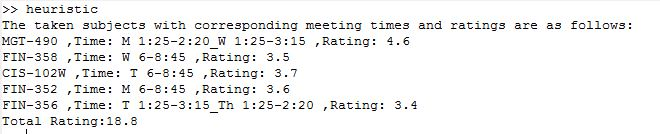
\includegraphics[width=0.8\textwidth]{heuristic}
    \caption{Output of Greedy Heuristic}
\end{figure}

The Octave code for greedy heuristic is attached in appendix part.\\
\newline
 \normalsize \textbf{a. LP:} 
Now I will use LP model to find an optimal solution. In my case it is a schedule that produces maximum rating. In other word I can say that I have to maximize.
\begin{center}
 $\sum\limits_{ij} c_{ij}x_{ij}$ where i = 1...10 and j = 1...8
\end{center}

Here c is matrix of coefficients  and x is matrix of decision variables. In this case Table 1 represents c and Table 2 represents x \\ 

\begin{table}[h]
\begin{center}
    \resizebox{0.95\textwidth}{!}{\begin{tabular}{| l | l | l | l | l | l | l | l | l |}
  
    \hline
    Meeting Time(s) & MGT 490 & FIN 358 & CIS 102T & CIS 102W & FIN 325 & FIN 352 & FIN 356 & FIN 359 \\ \hline
    M 6-8:45 p.m. & 1/0 & 1/0 & 1/0 & 1/0 & 1/0 & 1/0 & 1/0 & 1/0 \\ \hline
    T 6-8:45 p.m. & 1/0 & 1/0 & 1/0 & 1/0 & 1/0 & 1/0 & 1/0 & 1/0 \\ \hline
    W 6-8:45 p.m. & 1/0 & 1/0 & 1/0 & 1/0 & 1/0 & 1/0 & 1/0 & 1/0 \\ \hline
    F 6-8:45 p.m. & 1/0 & 1/0 & 1/0 & 1/0 & 1/0 & 1/0 & 1/0 & 1/0 \\ \hline
    \shortstack[l]{M 1:25-2:20 p.m. \\ W 1:25-3:15 p.m.} & 1/0 & 1/0 & 1/0 & 1/0 & 1/0 & 1/0 & 1/0 & 1/0 \\ \hline
    \shortstack[l]{T 1:25-3:15 p.m. \\ Th 1:25-2:20 p.m.} & 1/0 & 1/0 & 1/0 & 1/0 & 1/0 & 1/0 & 1/0 & 1/0 \\ \hline
    W 2:30-5:15 p.m. & 1/0 & 1/0 & 1/0 & 1/0 & 1/0 & 1/0 & 1/0 & 1/0 \\ \hline
    Th 2:30-5:15 p.m. & 1/0 & 1/0 & 1/0 & 1/0 & 1/0 & 1/0 & 1/0 & 1/0 \\ \hline
    Th 6-8:45 p.m. & 1/0 & 1/0 & 1/0 & 1/0 & 1/0 & 1/0 & 1/0 & 1/0 \\ \hline
    \shortstack[l]{M 1:25-3:15 p.m. \\ W 1:25-2:20 p.m.} & 1/0 & 1/0 & 1/0 & 1/0 & 1/0 & 1/0 & 1/0 & 1/0 \\ \hline
    
    \end{tabular}}
    \end{center}

\caption{Decision Variables}
\end{table}

If any course is taken in $(i,j)^{th}$ position the that  $x_{ij}$ is 1 otherwise it's 0. So my task is to maximaze $\sum\limits_{ij} c_{ij}x_{ij}$ which is actually sum of product of Table 1 and Table 2.

I used excel solver to solve the LP, unlike heuristic I had to introduce some other constraints. All the constraints that must meet to solve the LP are given bellow:

\begin{enumerate}[align=left,style=nextline,leftmargin=1.5cm,labelsep=\parindent,font=\normalfont]
\item[i.]  Each course cannot be taken more than once.
\item[ii.] Not more than one class can be chosen from one meeting time.
\item[iii.] There are some meeting times that conflicts with each other. Atmost one class can be taken from those conflicting time slots.  
\item[iv.] MGT 490 and FIN 358 must be taken.
\item[iv.] Number of course between CIS 102T and CIS 102W is one.
\item[v.] Number of courses between FIN 325, FIN 352, FIN 356 and FIN 359 is two.
\item[vi.] Total numer of course is five.
\end{enumerate}  

All the above mentioned constraints were added using excel solver. Here is an example how I added constraint in excel solver. Let us consider contraint (vi). There are four columns for FIN 325, FIN 352, FIN 356 and FIN 359. I must choose atmost two courses from these four. So summation of these four columns is equals to two and as I cannot take one coure more than once so summation of each column is less than or equal to zero. I added the other constraints similar way in excel solver. Meeting time contraints, Course conrtraints and resulting decision variables are shown in Figure 2,3 and 4.Objective function is sum of products of the elements of Table 1 and 2. After solving this problem in excel solver I get the optimal rating for this LP which is 19.5.         
\\\\\\\\\\\
 \normalsize \textbf{c. Extensions:}
In extentions part I will introduce new constraints to the LP part and observe what will happen to the optimal rating in extentions. The contraint is as follows:
\begin{enumerate}[align=left,style=nextline,leftmargin=1.5cm,labelsep=\parindent,font=\normalfont]
\item[i.]  Without lowering the maximum rating (19.5) too much Sarah wants to see whether she can attend classes only three days a week. 
\end{enumerate}

So I will have some new constraints as well as a new problem. The new problem is, I have to find in which days Sarah will take the classes as well as I will calculate the maximum rating as I calculated earlier. How I formulated and solved this extension is described bellow:\\
I have a new colums of decision variables. Each row of that column represents each day of a week. If one or more class is taken on a particular day then the cell is 1 otherwise it's 0. So I added this column as a decision varible in excel solver. (One thing I want to mention here that I kept the contraints and decision variables of the previous LP as it was and added the new decision variables and constraints for this extention.)
I added two constraints for this extension:\\
-Number of classes taken in a specific day of a week is less than or equals to 5.\\
- Total number of days in a week is 3.\\

For example I stored number of classes in each day of a week in a colum. Each row of that column actullay represents the sum of classes of that specific day. If any class is taken in a specific day of a week then the corresponding row of figure abc  will become 1 and the corresponding row in figure bcd must be less than or equals to 5. Finally total number of days in a week must be equal to 3. 

After adding the new dicision variables and constraints my set of previous decision variables is changed and it looks like as follows.
\\\\\\\\
The added decision variables is stated bellow.  
\\\\\\\\\
New Constraints
\\\\\\\
Finally I get new maximum rating after imposing three days a week restriction, which is 19.3. It is lower than 19.5 but not that much lower.   




%----------------------------------------------------------------------------------------

\end{document}